DP algorithms are obtained by turning the Bellman equations into assignments - update rules
for improving approximations in the future.

\section{Policy Evaluation (Prediction)}
\label{sec:policy_evaluation}
\emph{Policy evaluation} is the process of determining
$v_{\pi}(s), \forall s\in\mathcal{S}$.
\emph{Iterative policy evaluation} is the process of arbitrarily initializing the state-value
function for all states and then using the Bellman equation as an iterative update rule.
\begin{center}
    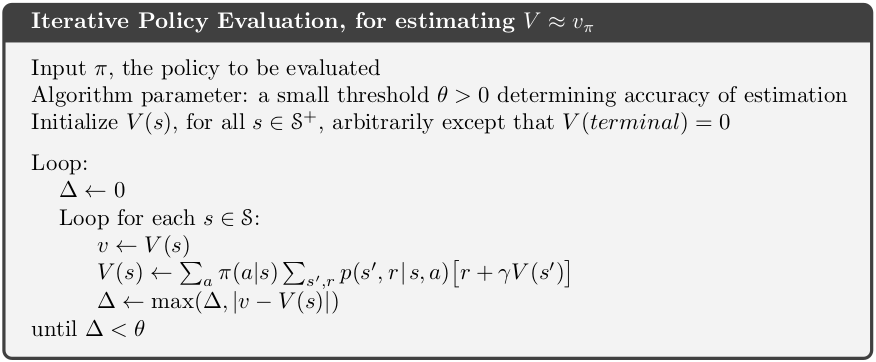
\includegraphics[width=\textwidth]{img/alg_iterative_policy_eval.png}
\end{center}

\section{Policy Improvement}
\label{sec:policy_improvement}
If we find policy $\pi'$ such that $q_{\pi'}(s,\pi'(s))\geq v_{\pi}(s)$ then we update
the policy $\pi$ so that $\pi(s)==\pi'(s)$.
At each step we select the action that appears best according to $q_{\pi}(s,a)$, the new
\textit{greedy} policy $\pi'$ is defined as the following:
\begin{myequation}{4.9}
    \begin{aligned}
        \pi'(s)&\doteq \argmax_a q_{\pi}(s,a) \\
        &=\argmax_a\sum_{s',r}p(s',r\mid s,a)\left[r+\gamma v_{\pi}(s')\right]
    \end{aligned}
\end{myequation}
\begin{itemize*}
    \item $\argmax_a$: value of $a$ for which the expression that follows is maximized.
\end{itemize*}
\emph{Policy improvement} is the process of making a new policy
that improves the original policy by making it greedy with respect to the value function of
the original policy.

\section{Policy Iteration}
\begin{center}
    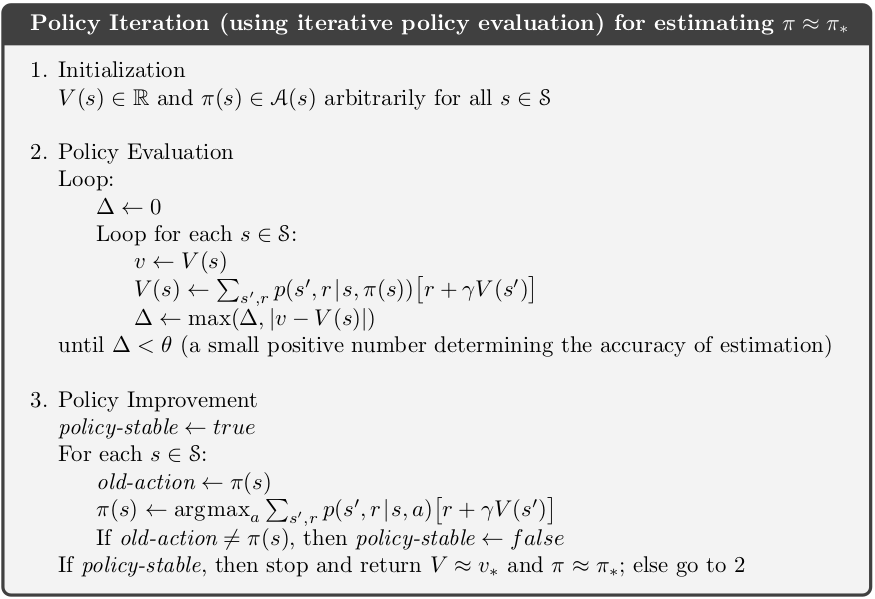
\includegraphics[width=\textwidth]{img/alg_iterative_policy_improvement.png}
\end{center}

\section{Value Iteration}
We are truncating \myref{sec:policy_evaluation}{policy evaluation} to get faster computation
but still ensure convergence.
Value iteration is truncating \myref{sec:policy_evaluation}{policy evaluation} to exactly one step.

\begin{myequation}{4.10}
    \begin{aligned}
        v_{k+1}(s)&\doteq\max_a\mathbb{E}\left[R_{t+1} + \gamma v_k(S_{t+1})\mid S_t=s,A_t=a\right] \\
        &=\max_a\sum_{s',r}p(s',r\mid s,a)\left[r+\gamma v_k(s')\right]
    \end{aligned}
\end{myequation}
\begin{center}
    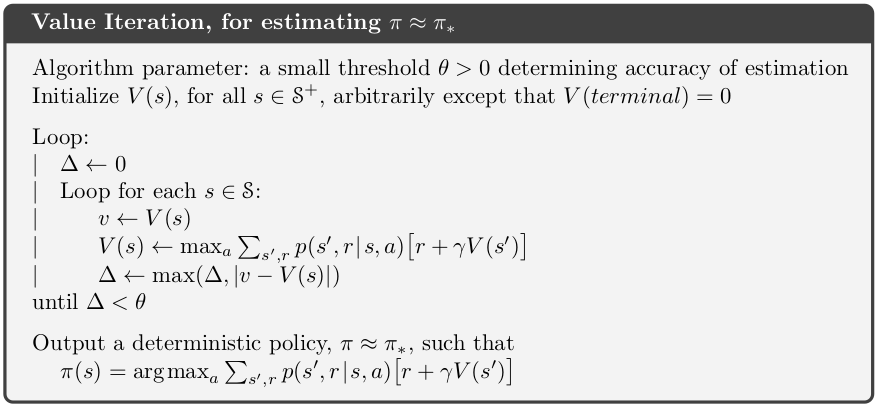
\includegraphics[width=\textwidth]{img/alg_value_iteration.png}
\end{center}

\section{Asynchronous Dynamic Programming}
These algorithms don't update all state values in each sweep but only target some.
This targeting can be done using the amount of update done in a sweep on a state, or given
preset priorities.
They also allow for real-time interaction - while an agent is playing the algorithm is running and learning.

\section{Generalized Policy Iteration (GPI)}
\label{sec:gpi}
\textit{Generalized Policy Iteration} (GPI) refers to a branch of algorithms
that allow for \myref{sec:policy_evaluation}{policy evaluation} and
\myref{sec:policy_improvement}{policy improvement} to intertwine.
\begin{center}
    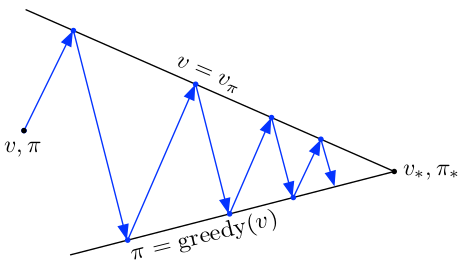
\includegraphics[scale=0.43]{img/general_policy_iteration_diagram.png}
\end{center}

\section{Efficiency of Dynamic Programming}

\section{Summary}
In this chapter we have become familiar with the basic ideas and algorithms of dynamic
programming as they relate to solving finite MDPs. Policy evaluation refers to the (typi-
cally) iterative computation of the value functions for a given policy. Policy improvement
refers to the computation of an improved policy given the value function for that policy.
Putting these two computations together, we obtain policy iteration and value iteration,
the two most popular DP methods. Either of these can be used to reliably compute
optimal policies and value functions for finite MDPs given complete knowledge of the
MDP.
Classical DP methods operate in sweeps through the state set, performing an expected
update operation on each state. Each such operation updates the value of one state
based on the values of all possible successor states and their probabilities of occurring.
Expected updates are closely related to Bellman equations: they are little more than
these equations turned into assignment statements. When the updates no longer result in
any changes in value, convergence has occurred to values that satisfy the corresponding
Bellman equation. Just as there are four primary value functions (v ⇡ , v ⇤ , q ⇡ , and q ⇤ ),
there are four corresponding Bellman equations and four corresponding expected updates.
An intuitive view of the operation of DP updates is given by their backup diagrams.
Insight into DP methods and, in fact, into almost all reinforcement learning methods,
can be gained by viewing them as generalized policy iteration (GPI). GPI is the general idea
of two interacting processes revolving around an approximate policy and an approximate
value function. One process takes the policy as given and performs some form of policy
evaluation, changing the value function to be more like the true value function for the
policy. The other process takes the value function as given and performs some form
of policy improvement, changing the policy to make it better, assuming that the value
function is its value function. Although each process changes the basis for the other,
overall they work together to find a joint solution: a policy and value function that are
unchanged by either process and, consequently, are optimal. In some cases, GPI can be
proved to converge, most notably for the classical DP methods that we have presented in
this chapter. In other cases convergence has not been proved, but still the idea of GPI
improves our understanding of the methods.
It is not necessary to perform DP methods in complete sweeps through the state
set. Asynchronous DP methods are in-place iterative methods that update states in an
arbitrary order, perhaps stochastically determined and using out-of-date information.
Many of these methods can be viewed as fine-grained forms of GPI.
Finally, we note one last special property of DP methods. All of them update estimates
of the values of states based on estimates of the values of successor states. That is, they
update estimates on the basis of other estimates. We call this general idea bootstrapping.
Many reinforcement learning methods perform bootstrapping, even those that do not
require, as DP requires, a complete and accurate model of the environment. In the next
chapter we explore reinforcement learning methods that do not require a model and do
not bootstrap. In the chapter after that we explore methods that do not require a model
but do bootstrap. These key features and properties are separable, yet can be mixed in
interesting combinations.
